\subsection{Remaining Work: Generating Descriptive Names Based on the Unique Attributes of Unit Tests}
\label{sec:remaining-work}

Finally, the first and second components of the second piece of my dissertation work were completed to provide necessary knowledge of if tests are often named after what makes them unique and how to extract unique attributes of tests.
%
Since the goal of the second piece of my dissertation work is to generate descriptive test names, as the last component, I plan to develop a new name generation approach to provide descriptive test names that are based primarily on unique attributes of tests.
%
This component will utilize the unique attributes of tests as the basis for its descriptive name generation process, and it completes the second piece of my dissertation work by generating descriptive test names.
%
The following subsections will describe my plan and timeline for completing this component.


\subsubsection{Research Plan}

The research plan of my dissertation work is described below.
%
For the first step of building the name generation approach, a further investigation of the tests that were categorized as partially named after what makes them unique will be conducted.
%
This step is to find the origin of additional attributes embedded in existing test names and check if it is possible to automate the process of extracting them from tests or other origin.
%
Based on the findings of the further investigation, I should be able to devise a method to extract them from tests or other origin as a set of additional attributes.
%
With the extraction method, it would be possible to include the additional attributes in the descriptive name generation process.


Second, using the unique and additional attributes as the basis of name generation, I will build a new name generation approach to provide descriptive test names.
%
To build the approach, I plan to look into the complex transformation process that convert the attributes of tests to descriptive test names.
%
For example, this transformation might require extracting certain words from the attributes, removing repetitive words in the attributes, or modifying certain phrases in the generated names, which would be preferred by developers.
%
Based on the this transformation, if a given test has non-descriptive name, my approach will transform the extracted attributes of it to a descriptive name for this test.


Last, the goal of the second piece of my dissertation work is to provide descriptive test names for developers, so I plan to evaluate the approach by both its coverage and effectiveness.
%
This approach is designed to be a fully automated process, so there is no human input needed (i.e., neither to detect poor names nor generate descriptive names).
%
For the coverage of my approach, I will check how often the approach can generate descriptive names for the test that are poorly named.
%
For the effectiveness, I will let software engineers to assess if they would prefer our generated names over the original names on a randomly selected set of tests with non-descriptive names.


The planned research questions in this step are:
%
\begin{enumerate}
    \item RQ1-Coverage: How often can the approach generate descriptive names for tests that are poorly named?
    \item RQ2-Effectiveness: Do the generated test names by the approach have developers approval?
\end{enumerate}
%
Also, a working prototype of the approach should be built before starting this evaluation.


\paragraph{Experimental Subjects}

For the experimental subjects, I plan to use a set of \num{6} open-source projects from Github\footnote{Same projects used for the evaluation in~\cref{sec:emp-eval-attributes}}.
%
These projects are randomly selected from the top \num{50} Java projects from Github~\cite{top50projects} (e.g., by the number of stars or watches), and each project involves with multiple developers.
%
Also, the unit tests from these projects are written by different developers at different times and cover a wide variety of application domains.
%
Hence, they tend to be more representative than other projects.
%
Moreover, these projects are different from the subjects we used in the empirical study in~\cref{sec:emp-study}, so I can prevent the threat of over-fitting towards the subjects of the empirical study.


\paragraph{RQ1-Coverage: How often can the approach generate descriptive names for tests that are poorly named?}

To answer RQ1, I plan to perform a quantitative analysis by calculating how often the approach can produce a descriptive name for the poorly named tests.
%
Because the usefulness of the approach depends on if it can generate descriptive names for tests that are poorly named, I need to look into this research question to measure the coverage of the approach.
%
To do that, I plan to extract a fixed number of randomly selected tests with non-descriptive names from each project and run the prototype on these tests for descriptive name generation.
%
Only two conditions could happen, either the approach can generate a descriptive name for a given test or not.
%
Therefore, the coverage of the approach will be determined by the number of tests that the approach can generate a descriptive name for versus the number of tests that the approach can not generate a descriptive name for.
%
Based on our preliminary observation, my approach should be able to cover nearly all of the poorly named tests and provide descriptive names for them.


\paragraph{RQ2-Effectiveness: Do the generated test names by the approach have developers approval?}

\begin{figure}[t]
    \centering
    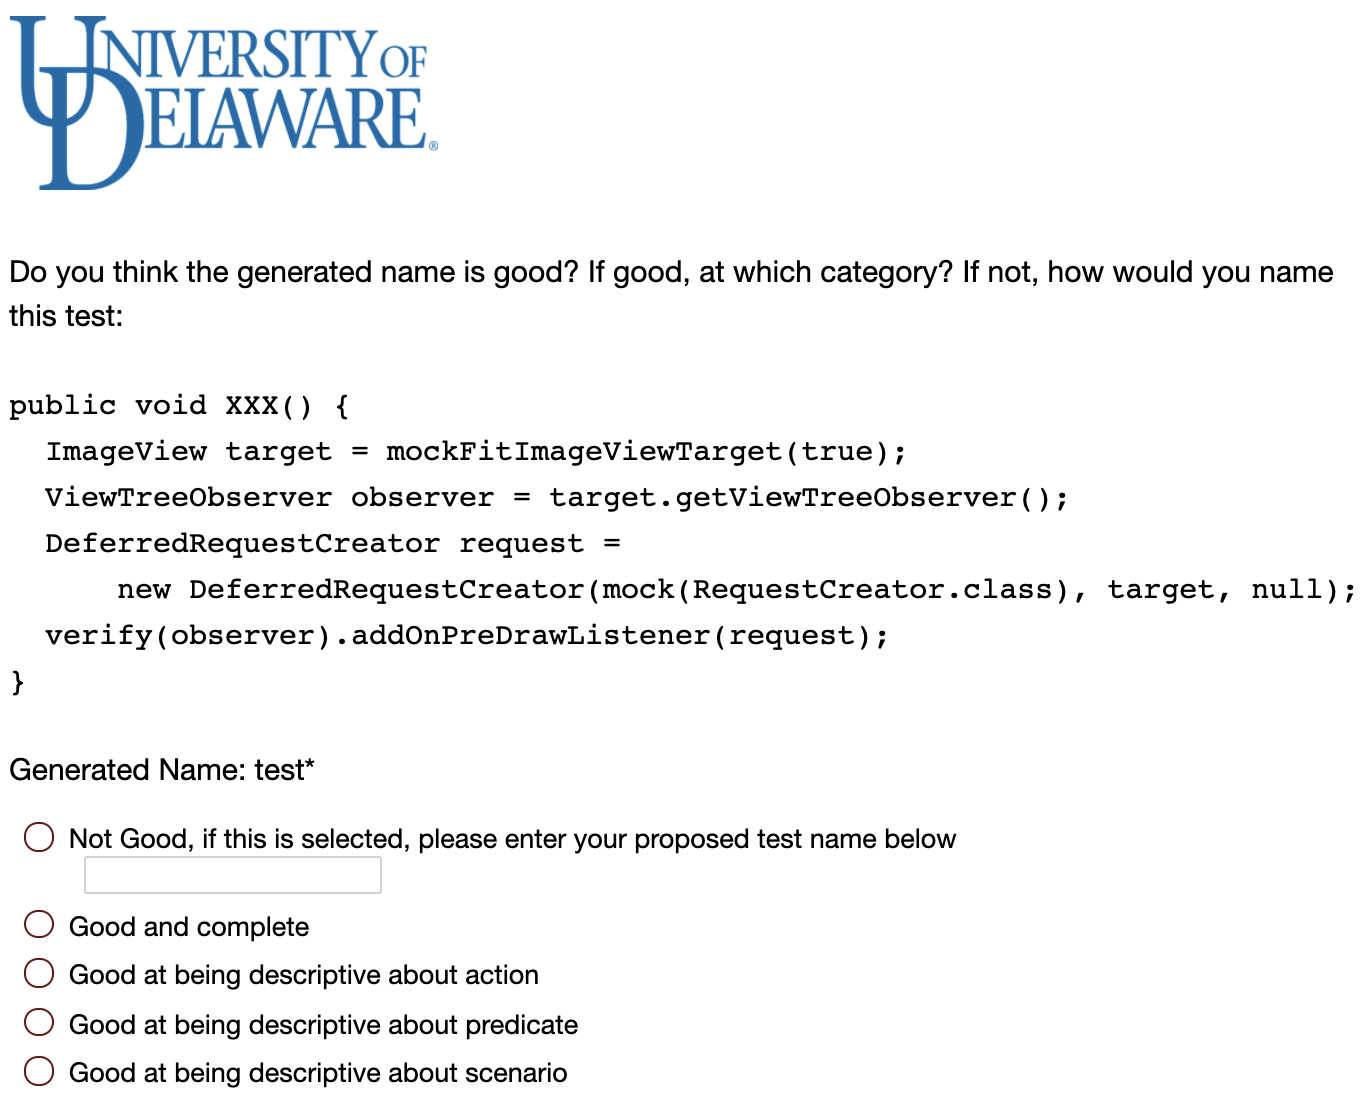
\includegraphics[scale=0.35]{figures/survey.png}
    \caption{Example of survey questions.}
    \label{fig:survey}
\end{figure}

To answer RQ2, I plan to conduct a developer-focused survey with a group of experienced developers (i.e., software engineers with at least three years of experience) by asking them if the generated names are descriptive about their corresponding tests, and
\begin{enumerate*}
    \item if yes, at which category would you put the generated name in
    \item if no, how would you name the corresponding test
\end{enumerate*}.
%
The goal of the approach is to provide descriptive test names for developers, so the best way to evaluate it is to ask developers if they would prefer its generated names when the original test names are non-descriptive.
%
Rather than using less credible participants (e.g., graduate students or random people from questions and answers websites), I will invite two experienced software engineers from \num{3} to \num{5} leading companies to our survey, which sums up to \num{6} to \num{10} developers in total.
%
To do that, I plan to use the results of RQ1, the randomly selected tests with non-descriptive names and their generated names, to form a survey for developers to answer.
%
For now, \num{15} tests with non-descriptive names are planned to be chosen from each project, which gives us a survey with \num{90} questions (i.e., about \num{30} minutes to complete).
%
For example of the survey questions, \cref{fig:survey} shows a survey question, which contains four categories if the generated name is good and ask developers to input their own names if the generated name does not meet their approval.
%
Each question contains a test body, our generated name for this test, while the original non-descriptive name is omitted.
%
And the current four categories are: descriptive and complete, descriptive at action of test, descriptive at predicate of test, and descriptive at scenario of test.
%
Because our approach is still in its early development stage, this survey is tentative and might be changed in the future.
%
The effectiveness of the approach is judged by if the majority of developers (i.e., \num{4} out of \num{6} or \num{7} out of \num{10}) would like to use our generated names for the tests and which category most generated names would be in (i.e., it could motivate us for future work).
%
Based the results of the empirical study in~\cref{sec:emp-study}, the new name generation approach should be able to provide descriptive test names that meet with developers approval.


\subsubsection{Proposed Timeline}

Currently, I already published the first piece of my dissertation work, which is a pattern-based approach to detect and improve non-descriptive test names~\cite{wu2020pattern}.
%
I also completed the first and second components of the second piece of my dissertation work, and they are submitted to ACM Transactions on Software Engineering and Methodology (TOSEM).
%
For my planned future work, I will start working on the last component of the second piece during Fall 2021 and complete this part by the end of Winter 2022.
%
Finally, my PhD dissertation defense is expected to be held during Spring 2022.